%% Commands for TeXCount
%TC:macro \cite [option:text,text]
%TC:macro \citep [option:text,text]
%TC:macro \citet [option:text,text]
%TC:envir table 0 1
%TC:envir table* 0 1
%TC:envir tabular [ignore] word
%TC:envir displaymath 0 word
%TC:envir math 0 word
%TC:envir comment 0 0

\documentclass[sigconf]{acmart}
%%
%% \BibTeX command to typeset BibTeX logo in the docs
\AtBeginDocument{%
  \providecommand\BibTeX{{%
    Bib\TeX}}}

\settopmatter{printacmref=false} % removes ACM reference format
\renewcommand\footnotetextcopyrightpermission[1]{} % removes footnote with conference info


\begin{document}

\title{SoccerCPD : Formation and Role Change-Point Detection in Soccer Matches Using Spatiotemporal Tracking Data}


\author{Fotios Kapotos}
\email{fotiskapotos@gmail.com}
\affiliation{%
  \institution{CentraleSupélec}
  \city{Gif-sur-Yvette}
  \country{France}
}

\author{Adonis Jamal}
\email{EMAIL}
\affiliation{%
  \institution{CentraleSupélec}
  \city{Gif-sur-Yvette}
  \country{France}
}

\begin{teaserfigure}
  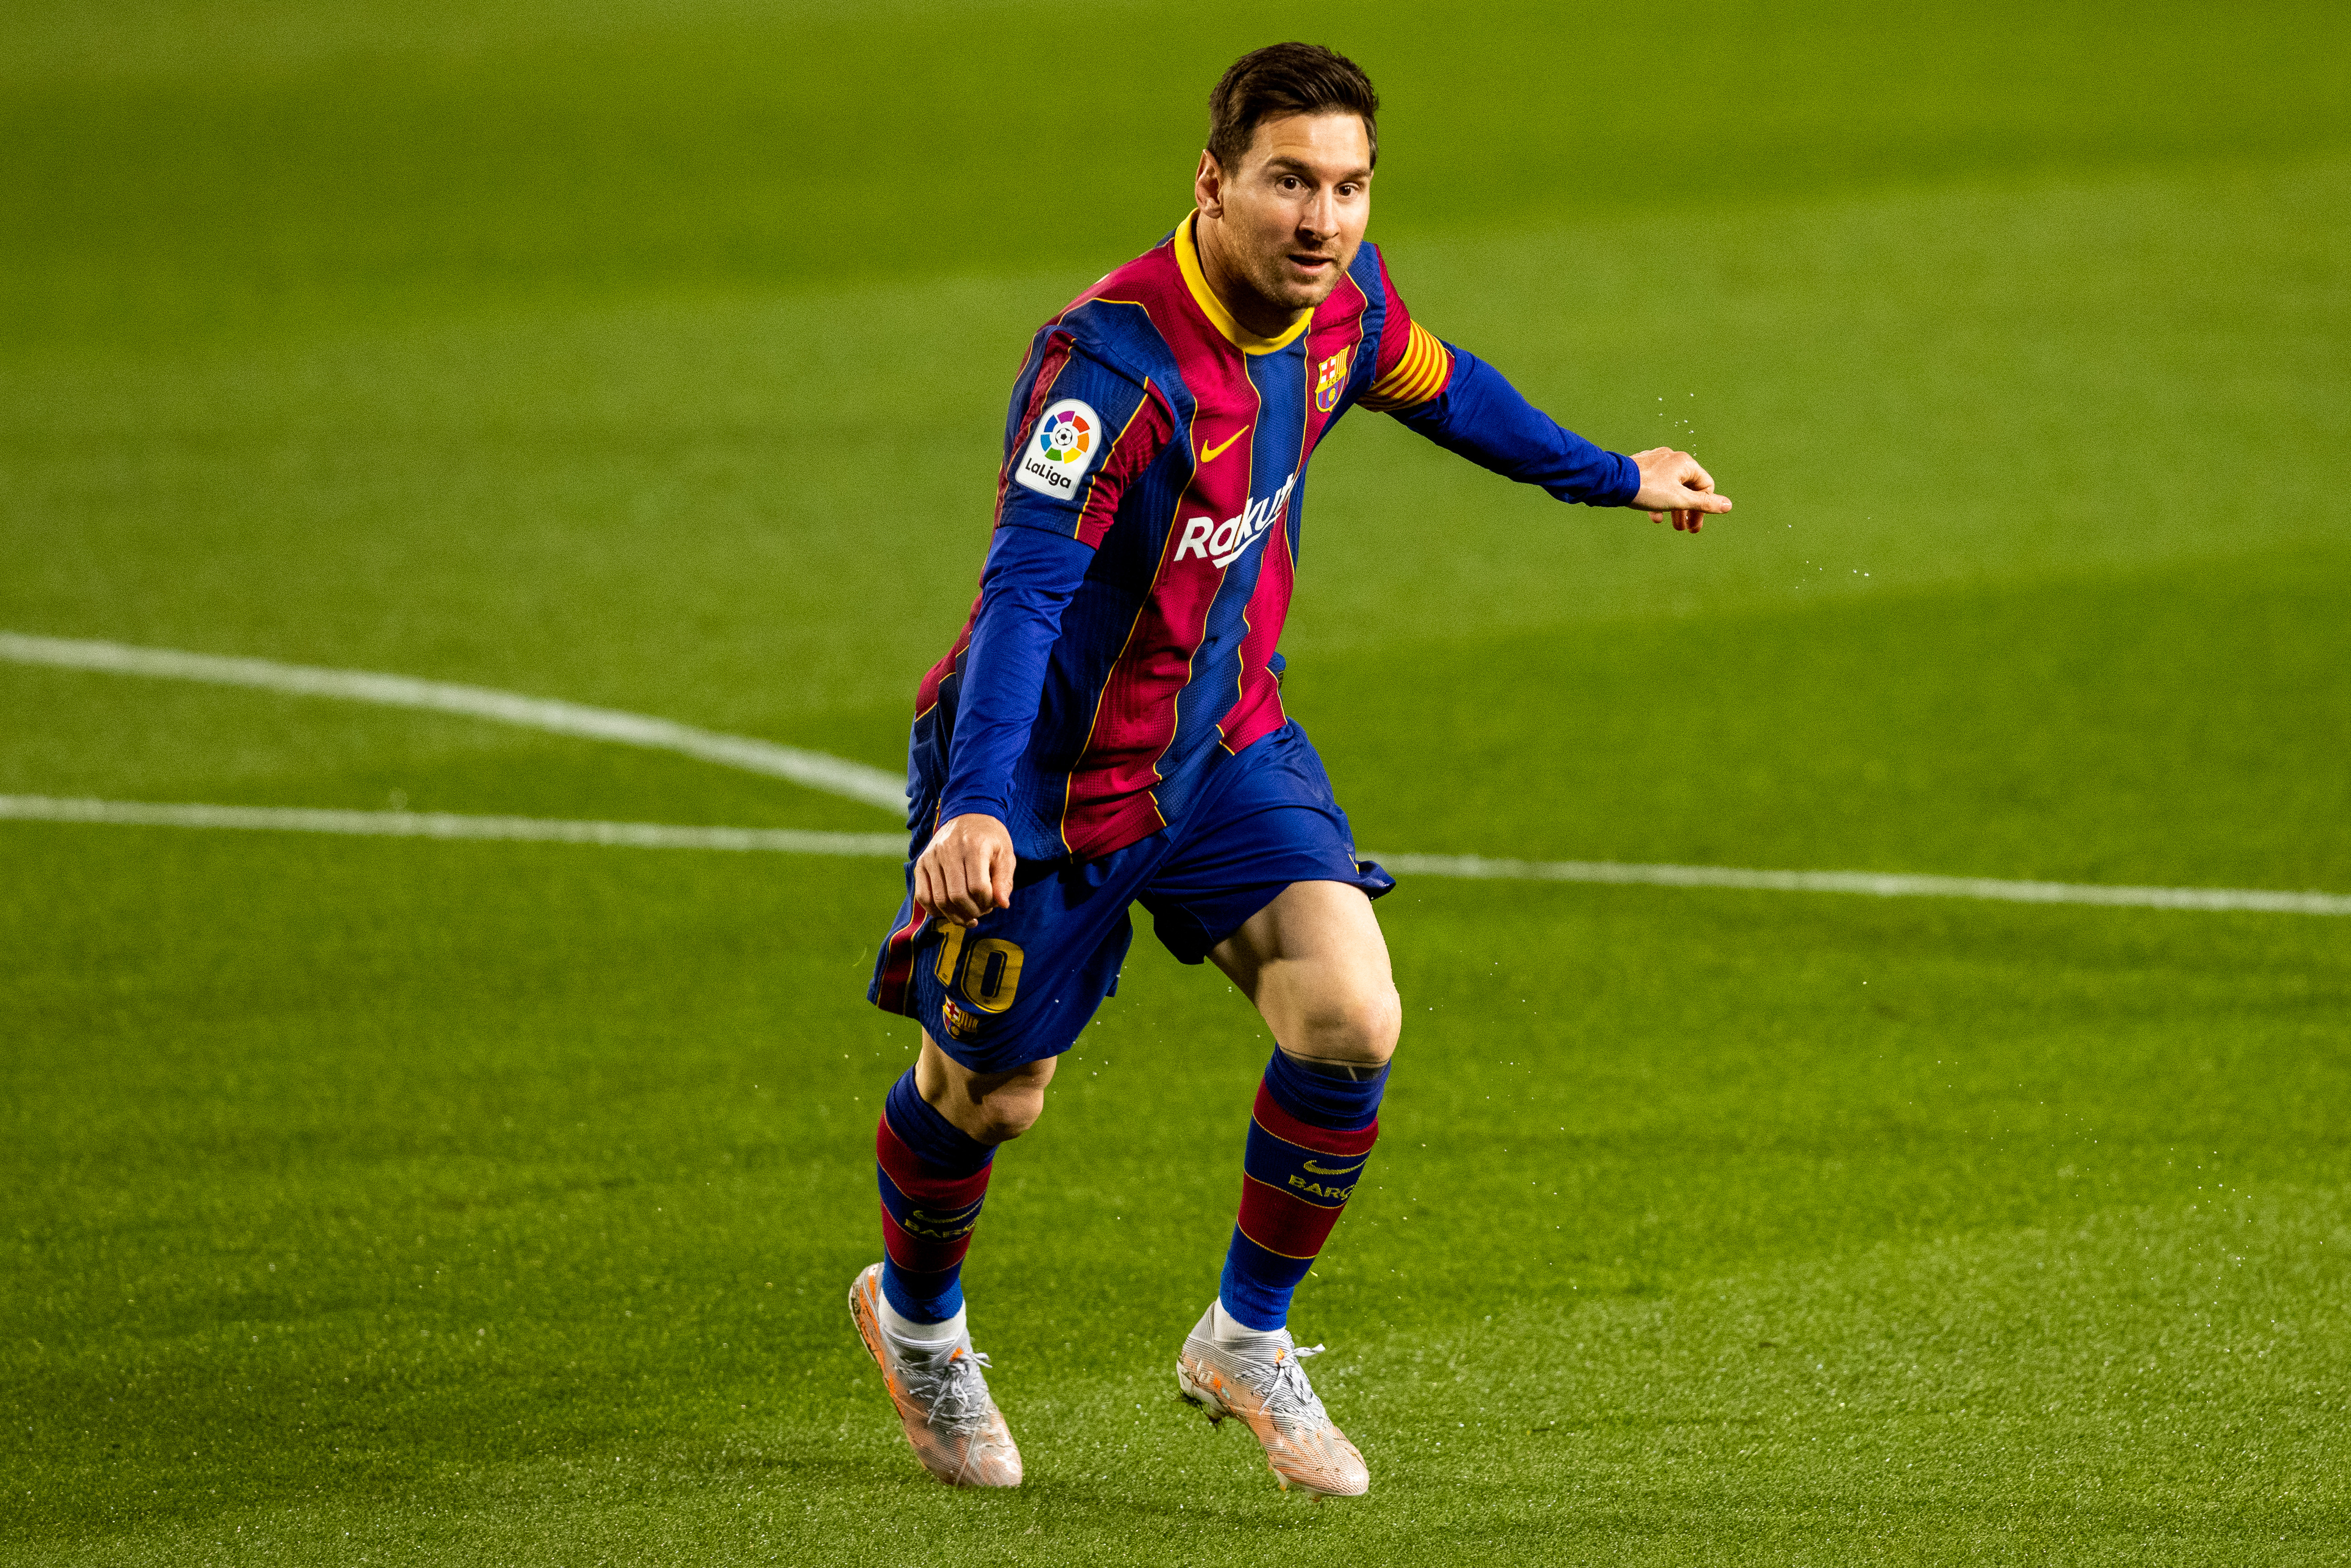
\includegraphics[width=\textwidth]{placeholder.jpg}
  \caption{Place Holder Image}
  \Description{Placeholder Image}
\label{fig:teaser}
\end{teaserfigure}



\begin{abstract}
  A clear and well-documented \LaTeX\ document is presented as an
  article formatted for publication by ACM in a conference proceedings
  or journal publication. Based on the ``acmart'' document class, this
  article presents and explains many of the common variations, as well
  as many of the formatting elements an author may use in the
  preparation of the documentation of their work.
\end{abstract}


\keywords{Do, Not, Use, This, Code, Put, the, Correct, Terms, for,
  Your, Paper}



%%
%% This command processes the author and affiliation and title
%% information and builds the first part of the formatted document.
\maketitle

\section{Introduction}
ACM's consolidated article template, introduced in 2017, provides a
consistent \LaTeX\ style for use across ACM publications, and
incorporates accessibility and metadata-extraction functionality
necessary for future Digital Library endeavors. Numerous ACM and
SIG-specific \LaTeX\ templates have been examined, and their unique
features incorporated into this single new template.

If you are new to publishing with ACM, this document is a valuable
guide to the process of preparing your work for publication. If you
have published with ACM before, this document provides insight and
instruction into more recent changes to the article template.

The ``\verb|acmart|'' document class can be used to prepare articles
for any ACM publication --- conference or journal, and for any stage
of publication, from review to final ``camera-ready'' copy, to the
author's own version, with {\itshape very} few changes to the source.


\section{}

%%
%% The next two lines define the bibliography style to be used, and
%% the bibliography file.
\bibliographystyle{ACM-Reference-Format}
\bibliography{bib}

\end{document}
\endinput
%%
%% End of file `sample-sigconf.tex'.
